\chapter{Fazit}
Von den anfänglichen Anforderungen und Ideen wurde tatsächlich ein großer Teil umgesetzt. Es kann also mit verschiedensten nützlichen UI-Elementen online mit Anderen gespielt werden. Was bisher nicht umgesetzt wurde ist insbesondere eine schöne graphische Oberfläche zur Darstellung des Statistiken. Alle hierfür benötigten Daten werden allerdings bereits in der Datenbank erfasst und können daher in einer späteren Version noch mit einer entsprechenden API Funktion und einem Bereich im Frontend dargestellt werden. Außerdem wurde zwar eine Kalenderfunktion zum Planen gemeinsamer Spieltermine implementiert, allerdings noch nicht vollständig an ein automatisiertes Benachrichtigungssystem angebunden. Zwar sind auch dafür bereits Ansätze von entsprechenden Bot-Implementierungen vorhanden, diese müssten allerdings noch fertiggestellt und an den Kalender angebunden werden. Und auch das Feature des teil-automatischen Ausspielens einer Karte ist aktuell nicht implementiert. Jedoch wurden auch insbesondere im Bereich der GUI einige Features wesentlich detaillierter als zu Beginn gefordert ausgearbeitet. Beispiele dafür sind der "Dark-Mode" (vergleiche \cref{fig:menu} und \cref{fig:menu-light}), die Animationen bei der Kartenauswahl oder die personalisierbaren Benachrichtigungseinstellungen (siehe \cref{fig:sound}).

\begin{figure}[h]
	\centering
	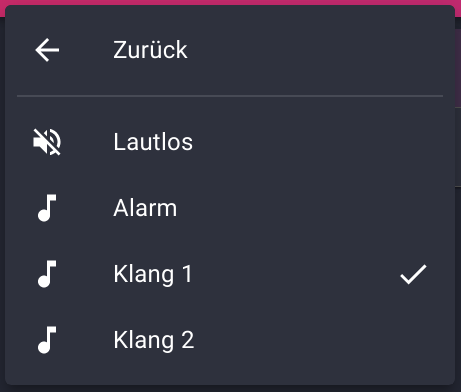
\includegraphics[height=5cm]{images/sound.png}
	\caption{Benachrichtigungseinstellungen}
	\label{fig:sound}
\end{figure}

Aufgrund der vielen Ideen wurde, wie bereits im letzten Abschnitt zu erahnen ist, ein starker Fokus auf die Implementierung neuer Features gelegt, wodurch Themen wie Code-Dokumentation und ein durchdachtes und übersichtliches Logging in den Hintergrund gerückt sind und daher noch ausgebaut werden können. Außerdem wurden kaum Tests entwickelt. Dies war aber eher unproblematisch, da das aktive Testen der Anwendung, also deren Nutzung, kein Problem war und ausführlich praktiziert wurde.

Zusammengefasst wurde das Projekt also mit einem den Anforderungen gerechten Ergebnis erfolgreich durchgeführt. Dabei konnten zwar nicht alle Ideen umgesetzt werden und einige Punkte wurden nur begrenzt betrachtet, aber es ist eine solide Web-Anwendung entstanden, welche ihren grundlegenden Zweck vollständig erfüllt und Spielraum für eine zukünftige Weiterentwicklung bietet.
